
\documentclass[12pt,a4paper]{article}
\usepackage[utf8]{inputenc}
\usepackage[T1]{fontenc}
\usepackage{lmodern}
\usepackage[spanish,es-nodecimaldot]{babel}
\usepackage[a4paper,margin=2.5cm]{geometry}
\usepackage{booktabs}
\usepackage{amsmath}
\usepackage{float}
\usepackage{graphicx}
\usepackage{tabularx}
\usepackage{hyperref}
\hypersetup{colorlinks=true,linkcolor=black,urlcolor=blue,pdftitle={Comparación de algoritmos de clasificación supervisada sobre Seismic-Bumps}}
\title{Informe de avance\\[0.75em]Clasificación supervisada de eventos sísmicos peligrosos en minería subterránea: comparación de árbol de decisión, Naive Bayes, k-NN y regresión logística}
\author{Martinez Mauricio Leonel\\DNI: 45.549.925}
\date{2026}
\begin{document}
\maketitle

\section{Introducción}
La minería subterránea puede estar expuesta a eventos sísmicos de alta energía que representan un riesgo para la seguridad de los trabajadores, la infraestructura y la continuidad de las operaciones. Estos eventos pueden producir desprendimientos, daños materiales, interrupciones de la actividad y condiciones de trabajo que requieren una respuesta rápida. En este contexto, la disponibilidad de registros históricos de actividad sísmica y sismoacústica permite estudiar si los patrones observados durante un turno contienen información útil para anticipar el nivel de peligrosidad del turno siguiente.

Este informe presenta el estado de avance de un estudio de clasificación supervisada aplicado al conjunto de datos \textit{Seismic-Bumps}. El problema se formula como una clasificación binaria: cada instancia se asigna a una clase no peligrosa o a una clase peligrosa. El alcance del proyecto integrador comprende la comparación de cuatro algoritmos: árbol de decisión, Naive Bayes, k-NN y regresión logística. En esta versión se encuentran disponibles resultados empíricos de los cuatro modelos base planificados. La evaluación no se limita a la exactitud global, porque la clase peligrosa es minoritaria y, por lo tanto, un clasificador que favorezca sistemáticamente la clase mayoritaria puede presentar una exactitud elevada sin detectar una proporción suficiente de los eventos relevantes.

El objetivo de esta etapa no es presentar todavía un modelo final para uso operativo ni seleccionar un algoritmo entre los cuatro planificados, sino establecer una línea de base empírica, documentar el comportamiento de los primeros clasificadores y dejar identificados los aspectos que requieren profundización. En particular, se busca observar la relación entre rendimiento global, discriminación medida mediante AUC y capacidad de detección de la clase peligrosa. Esta lectura conjunta resulta necesaria para evitar conclusiones basadas en una única métrica.

\section{Problema y pregunta de investigación}
La tarea se formula como un problema de clasificación binaria sobre registros de actividad sísmica. La etiqueta \texttt{class} toma el valor 0 para un registro no peligroso y el valor 1 para un registro peligroso. El interés práctico se encuentra en la clase 1, ya que sus errores de omisión pueden tener un costo mayor que los errores asociados a la emisión de una alerta innecesaria.

El problema central consiste en determinar si los 18 atributos predictivos disponibles permiten distinguir de manera útil ambas clases y qué comportamiento presentan el árbol de decisión, Naive Bayes, k-NN y la regresión logística bajo un procedimiento de evaluación común. La dificultad principal surge de la distribución desigual de la variable objetivo: la clase 0 reúne la gran mayoría de los registros, mientras que la clase 1 representa una proporción reducida. En consecuencia, la exactitud debe interpretarse junto con la matriz de confusión y con métricas específicas de la clase positiva.

La pregunta de investigación que orienta el trabajo es:
\begin{quote}
¿Qué diferencias presentan un árbol de decisión, Naive Bayes, k-NN y regresión logística en términos de rendimiento global y detección de la clase peligrosa en el conjunto Seismic-Bumps, bajo un procedimiento de evaluación común?
\end{quote}
Esta formulación conserva el alcance original del proyecto integrador. La presente versión informa la evidencia disponible para el árbol de decisión base, Naive Bayes base, k-NN con $k=5$ y regresión logística.

\section{Objetivos}
El objetivo general es analizar comparativamente el comportamiento de un árbol de decisión, Naive Bayes, k-NN y regresión logística para clasificar la ocurrencia de eventos sísmicos peligrosos en el conjunto Seismic-Bumps.

Los objetivos específicos son:
\begin{itemize}
\item describir el tamaño, la estructura y la distribución de clases del conjunto de datos;
\item establecer un procedimiento reproducible de evaluación mediante validación cruzada estratificada;
\item configurar y evaluar los cuatro algoritmos planificados mediante un procedimiento común;
\item documentar los resultados obtenidos en Altair AI Studio para los cuatro modelos base ejecutados;
\item analizar las matrices de confusión con filas verdaderas y columnas predichas;
\item comparar exactitud, AUC, precisión, recall y F1 de la clase peligrosa sin reducir la evaluación a una sola métrica;
\item interpretar las diferencias entre rendimiento global y capacidad de detección de la clase minoritaria; y
\item construir una comparación conjunta de los cuatro algoritmos sin reducir la selección a una única métrica.
\end{itemize}

\section{Descripción del conjunto de datos}
Se utilizó el conjunto \textit{Seismic-Bumps}, disponible en el repositorio público UCI Machine Learning Repository. El archivo local utilizado en el flujo de trabajo es \texttt{seismic-\allowbreak bumps.arff}. El conjunto contiene 2584 instancias y 19 atributos en total: 18 atributos predictivos y una variable objetivo denominada \texttt{class}. En la inspección realizada no se detectaron valores faltantes.

\begin{table}[H]
\centering
\caption{Características generales del conjunto de datos.}
\label{tab:dataset-general}
\begin{tabular}{ll}
\toprule
\textbf{Característica} & \textbf{Descripción} \\
\midrule
Nombre & Seismic-Bumps \\
Instancias & 2584 \\
Atributos totales & 19 \\
Atributos predictivos & 18 \\
Variable objetivo & \texttt{class} \\
Formato & ARFF \\
Valores faltantes & No detectados \\
\bottomrule
\end{tabular}
\end{table}

La distribución de la variable objetivo muestra un desbalance marcado. La clase 0 contiene 2414 instancias, equivalentes al 93,42\% del conjunto, mientras que la clase 1 contiene 170 instancias, equivalentes al 6,58\%. Esta diferencia debe ser tenida en cuenta en la interpretación: un modelo puede acertar una gran cantidad de registros de la clase 0 y, al mismo tiempo, omitir la mayoría de los casos de la clase 1.

\subsection{Tratamiento del desbalance}
La distribución observada equivale aproximadamente a una relación de 14,2 registros de la clase 0 por cada registro de la clase 1. En este contexto, la exactitud puede resultar engañosa: un clasificador que predijera casi siempre la clase mayoritaria podría alcanzar una proporción elevada de aciertos y, sin embargo, detectar muy pocos eventos peligrosos. Por ello, la evaluación deberá considerar especialmente la capacidad de identificar la clase 1, junto con el costo asociado a los falsos positivos y falsos negativos.

Como extensión complementaria y futura se prevé evaluar el uso de SMOTE (Synthetic Minority Over-sampling Technique), propuesto por Chawla et al. (2002). SMOTE genera ejemplos sintéticos de la clase minoritaria a partir de la combinación de observaciones existentes y sus vecinos cercanos; por lo tanto, los nuevos registros no son observaciones reales del conjunto original, sino construcciones artificiales destinadas a mejorar la representación de la clase 1 durante el entrenamiento. A diferencia del submuestreo, que reduce la cantidad de observaciones de la clase mayoritaria y puede descartar información, SMOTE conserva esas observaciones. También se diferencia del oversampling aleatorio, que replica registros minoritarios existentes, mientras que SMOTE busca generar nuevas muestras sintéticas. Esta extensión no reemplaza la comparación prevista entre árbol de decisión, Naive Bayes, k-NN y regresión logística.

Si se implementa, la aplicación de SMOTE se limitará exclusivamente al subproceso de entrenamiento de cada partición de la validación cruzada. De este modo, los ejemplos sintéticos se generarán únicamente a partir de los datos utilizados para entrenar en cada partición, evitando que información del conjunto de prueba influya en el ajuste del modelo. El conjunto de prueba conservará la distribución original del conjunto, sin aplicar SMOTE, para que la evaluación represente la frecuencia de clases observada en los datos. La comparación principal deberá completarse primero con los cuatro algoritmos planificados; luego, SMOTE podrá analizarse como una extensión separada frente a las respectivas líneas de base.

El uso de SMOTE también introduce riesgos metodológicos que deberán ser examinados. Los ejemplos sintéticos pueden amplificar ruido, generar observaciones en regiones de solapamiento entre clases o favorecer un aumento de falsos positivos. Por esta razón, SMOTE se incorporará como una alternativa experimental y no como una mejora asumida de antemano; sus resultados deberán interpretarse conjuntamente con la matriz de confusión, el recall, la precisión, el F1 y el AUC.

\begin{table}[H]
\centering
\caption{Distribución de la variable objetivo.}
\label{tab:class-distribution}
\begin{tabular}{lrr}
\toprule
\textbf{Clase} & \textbf{Cantidad} & \textbf{Proporción} \\
\midrule
No peligrosa (0) & 2414 & 93,42\% \\
Peligrosa (1) & 170 & 6,58\% \\
\midrule
Total & 2584 & 100,00\% \\
\bottomrule
\end{tabular}
\end{table}

\begin{figure}[H]
\centering
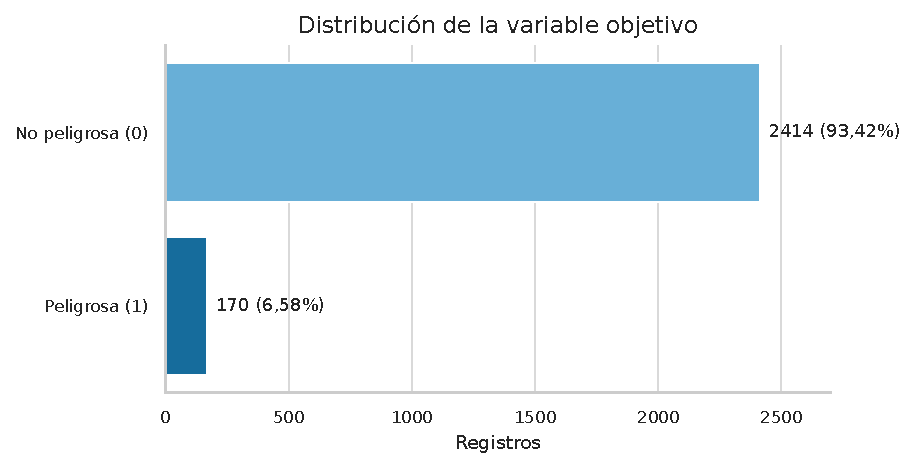
\includegraphics[width=0.78\textwidth]{output/figures/distribucion_clases.pdf}
\caption{Distribución de las clases del conjunto Seismic-Bumps.}
\label{fig:class-distribution}
\end{figure}

Los atributos describen condiciones y mediciones asociadas con la actividad registrada durante los turnos. La variable objetivo resume la ocurrencia de un evento clasificado como peligroso. En esta etapa, el conjunto se utiliza como fuente de observaciones históricas para comparar algoritmos; no se afirma todavía que la relación observada sea suficiente para una implementación de alerta en tiempo real.

\section{Plan de análisis}
El plan de análisis se organiza en cuatro etapas. Primero, se verifica la estructura del archivo ARFF, el número de instancias, la cantidad de atributos, la ausencia de valores faltantes y la distribución de la clase objetivo. Segundo, se configuran el árbol de decisión, Naive Bayes, k-NN y la regresión logística en Altair AI Studio con los mismos datos y el mismo esquema de evaluación. Tercero, se examinan las matrices de confusión y las métricas globales y de clase de cada algoritmo. Finalmente, se realiza una interpretación conjunta que distingue la exactitud de la capacidad efectiva para detectar la clase peligrosa.

Todos los resultados empíricos presentados fueron obtenidos mediante Altair AI Studio utilizando validación cruzada estratificada de 10 particiones. La estratificación busca conservar, dentro de cada partición, una representación comparable de las dos clases. De esta forma, las métricas reportadas reflejan el comportamiento promedio del procedimiento sobre diferentes particiones y no el desempeño en una única división arbitraria del conjunto.

Las matrices se expresan con filas verdaderas y columnas predichas. En esta convención, para la clase 1 se definen los verdaderos positivos como los registros peligrosos correctamente identificados, los falsos negativos como los registros peligrosos clasificados como no peligrosos y los falsos positivos como los registros no peligrosos clasificados como peligrosos. Las métricas agregadas se calculan a partir de la matriz total:
\[
\mathrm{precision}=\frac{TP}{TP+FP},\qquad
\mathrm{recall}=\frac{TP}{TP+FN},
\]
\[
\mathrm{F1}=\frac{2\cdot\mathrm{precision}\cdot\mathrm{recall}}
{\mathrm{precision}+\mathrm{recall}}.
\]
Además de los valores agregados, se consignan cuando están disponibles los valores del encabezado de AI Studio y su variabilidad entre particiones. Esta distinción es importante: los promedios informados por la herramienta y los cocientes calculados a partir de la matriz acumulada no necesariamente coinciden exactamente, porque se obtienen mediante operaciones diferentes.

\begin{figure}[H]
\centering
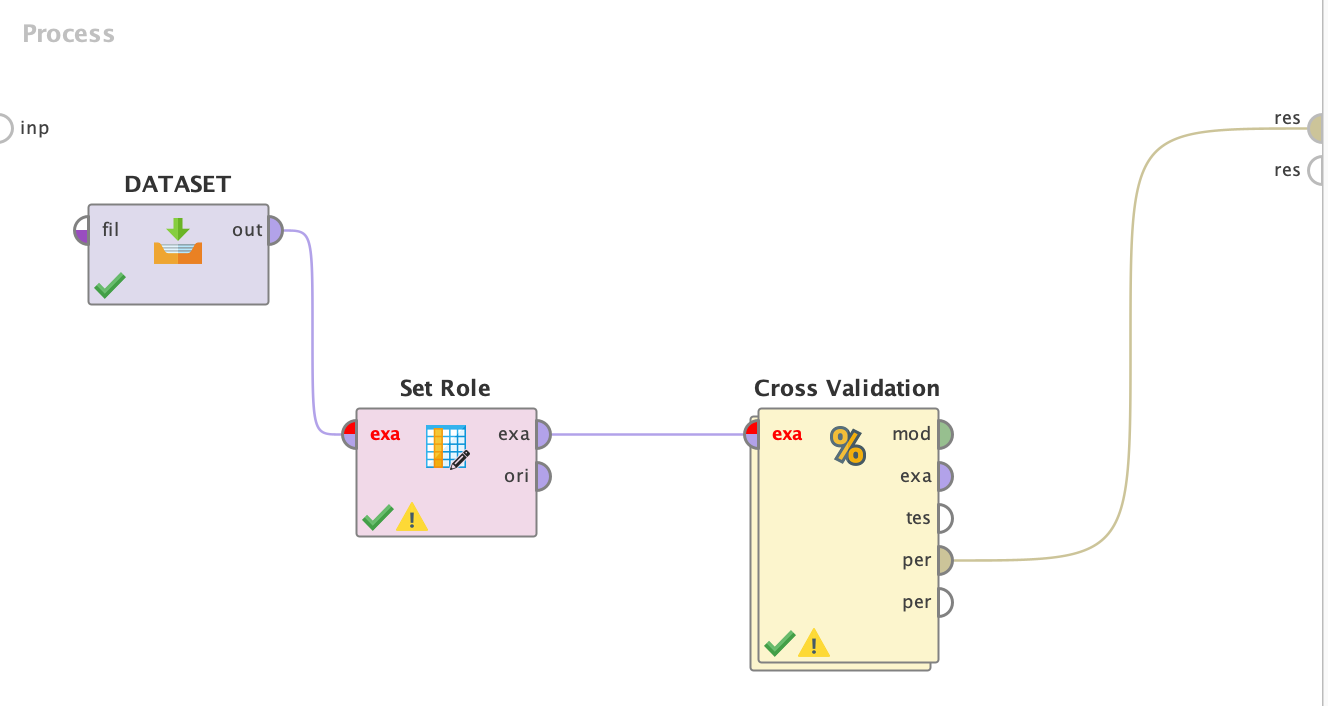
\includegraphics[width=0.88\textwidth]{output/figures/proceso_ai_studio_user.png}
\caption{Esquema del proceso de trabajo utilizado para obtener los resultados mediante Altair AI Studio.}
\label{fig:ai-studio-process}
\end{figure}

\begin{figure}[H]
\centering
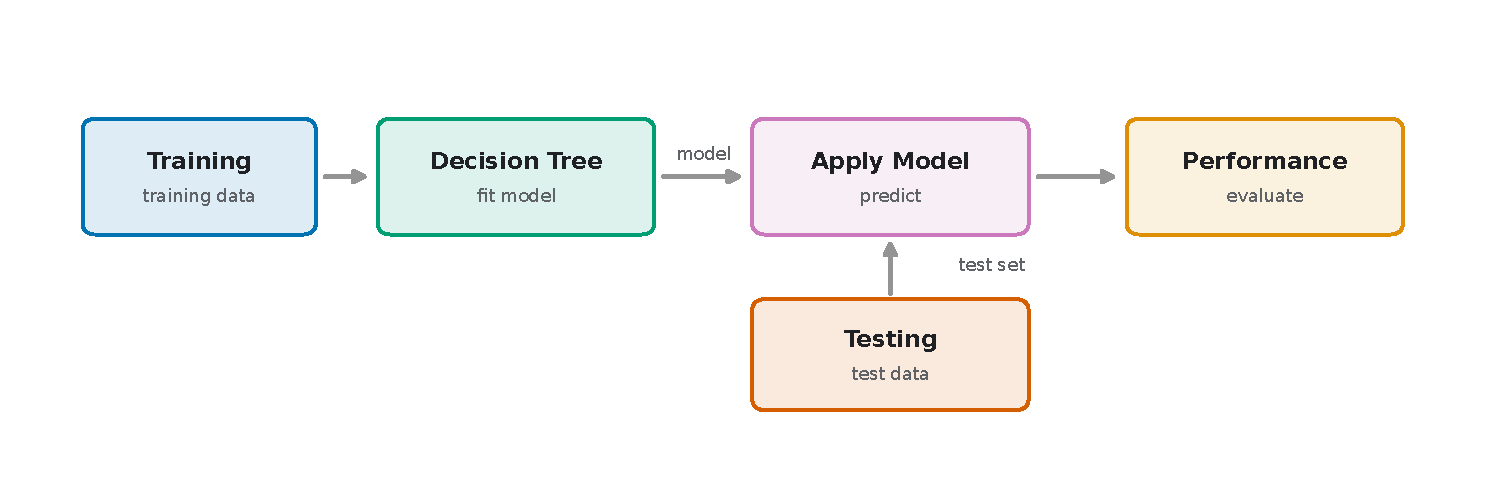
\includegraphics[width=0.88\textwidth]{output/figures/proceso_cross_validation_clean.pdf}
\caption{Esquema de la validación cruzada estratificada utilizada en la evaluación.}
\label{fig:cross-validation-process}
\end{figure}

\section{Implementación y configuración de k-NN}
El algoritmo k-NN se incorporó al flujo de evaluación como el tercer modelo analizado. Debido a que este método clasifica una instancia a partir de la proximidad de sus vecinos, la escala de las variables numéricas afecta directamente el cálculo de las distancias. En el conjunto \textit{Seismic-Bumps}, las variables numéricas no se encuentran necesariamente en el mismo rango; por este motivo, una variable con valores de mayor magnitud podría dominar la medida de distancia aunque no fuera la más informativa para la clasificación.

Para reducir este efecto se utilizó el operador \textit{Normalize} antes de k-NN. La normalización transforma las variables numéricas a una escala comparable y evita que las diferencias de magnitud determinen por sí solas qué observaciones se consideran cercanas. La transformación se ajusta dentro del subproceso de entrenamiento de cada partición de la validación cruzada, de manera que los parámetros calculados a partir del conjunto de entrenamiento no incorporen información del conjunto de prueba.

La salida \texttt{pre} de \textit{Normalize} se conectó a \textit{Group Models} junto con el modelo generado por k-NN. Este operador agrupa el modelo de preprocesamiento y el clasificador en un único modelo compuesto. Así, al aplicar el modelo a datos no vistos, primero se reproduce la misma transformación de normalización y luego se ejecuta la clasificación k-NN. Esta conexión evita que el modelo se entrene con datos normalizados y se aplique a datos de prueba en una escala diferente, y mantiene el preprocesamiento dentro del ciclo de validación cruzada. La Figura~\ref{fig:knn-normalize-group-models} muestra el flujo implementado.

\begin{figure}[H]
\centering
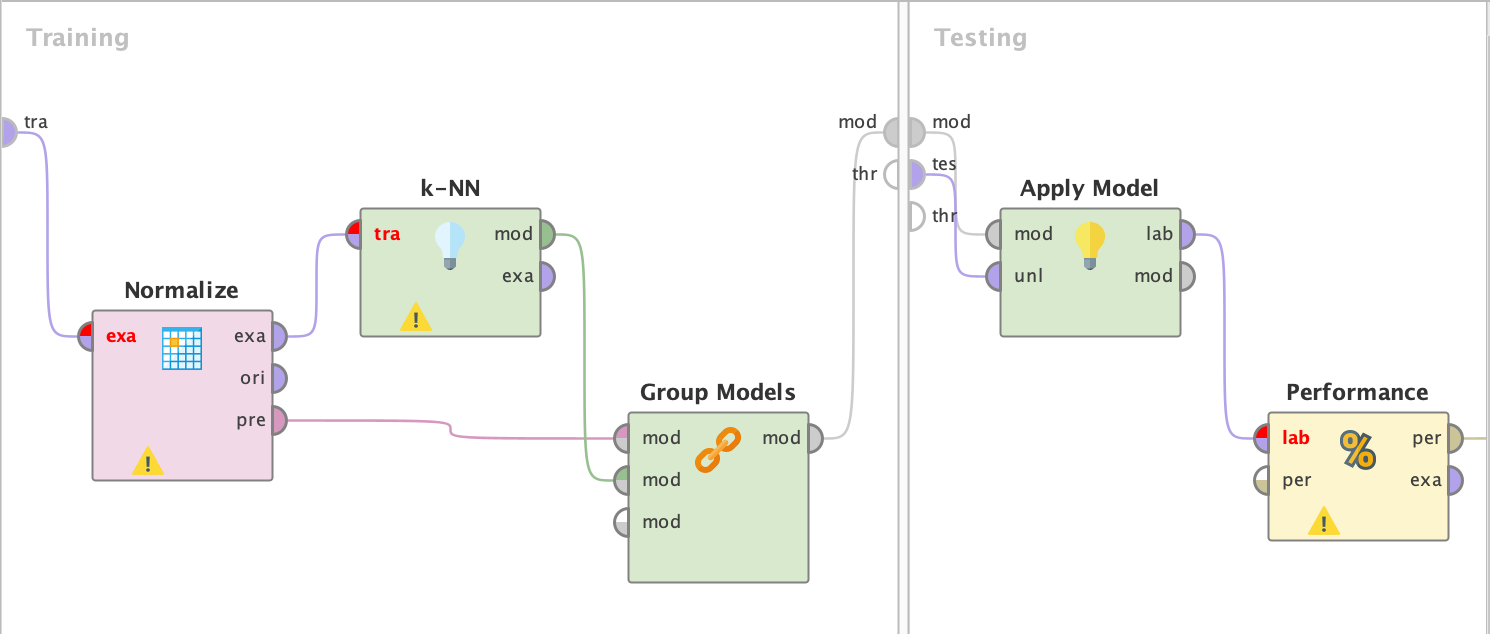
\includegraphics[width=0.98\textwidth]{output/figures/knn_normalize_group_models.png}
\caption{Flujo de k-NN con normalización y agrupación del modelo de preprocesamiento mediante \textit{Group Models}.}
\label{fig:knn-normalize-group-models}
\end{figure}

El parámetro $k$ se evaluó con los valores impares 3, 5, 7 y 9. En todos los casos se mantuvieron constantes el conjunto de datos, la normalización, la validación cruzada estratificada de 10 particiones y el resto del flujo. Los resultados se compararon priorizando la detección de la clase 1, sin dejar de considerar la precisión, el F1, la exactitud y el AUC informado por AI Studio.

\section[Implementación y configuración de la regresión logística]{Implementación y configuración de la regresión\\logística}
La regresión logística se implementó mediante el operador \textit{Generalized Linear Model} con familia binomial. Esta formulación utiliza el enlace logit para relacionar linealmente los atributos con el logaritmo de las probabilidades relativas de pertenecer a la clase 1. En consecuencia, el modelo estima la probabilidad de que un registro corresponda a la clase peligrosa y la transforma en una decisión de clase mediante el umbral utilizado por AI Studio.

El modelo se entrenó dentro del subproceso de entrenamiento de una validación cruzada estratificada de 10 particiones. En cada iteración, el \textit{Generalized Linear Model} se ajustó únicamente con nueve particiones y su salida se aplicó a la partición de prueba mediante \textit{Apply Model}. Luego, el operador \textit{Performance} calculó la matriz de confusión y las métricas correspondientes. La Figura~\ref{fig:logistic-cross-validation} muestra este flujo. SMOTE no forma parte de esta ejecución base y permanece reservado como una extensión experimental posterior.

\begin{figure}[htbp]
\centering
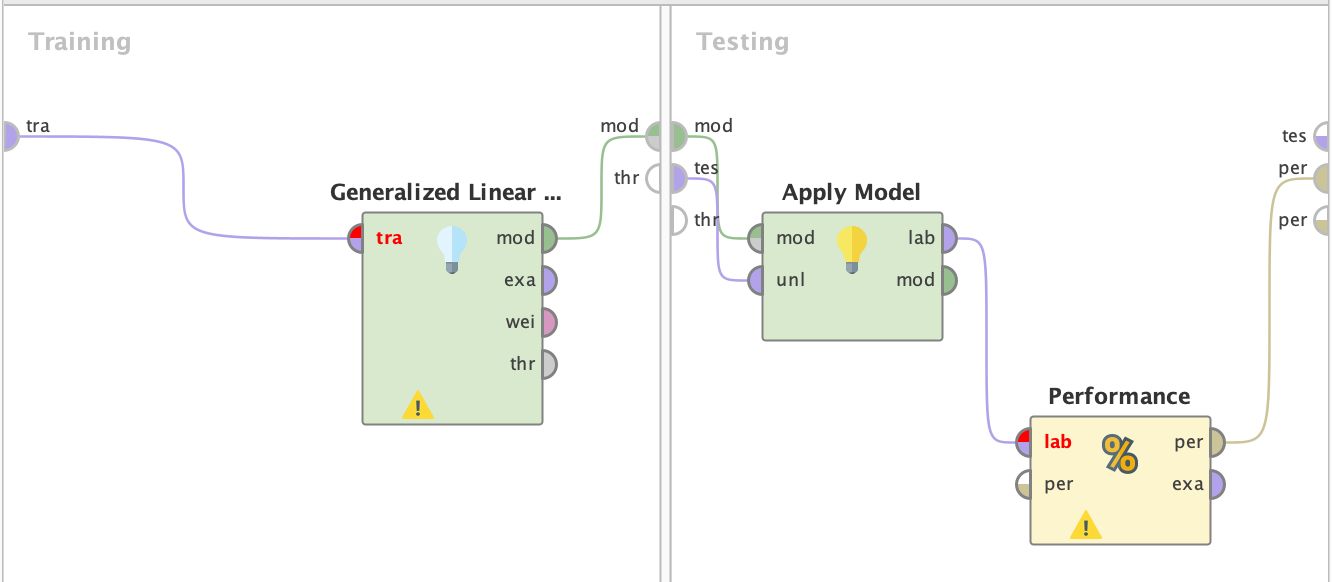
\includegraphics[width=0.98\textwidth]{output/figures/logistic_regression_cross_validation_user.png}
\caption{Flujo de entrenamiento y prueba de la regresión logística mediante \textit{Generalized Linear Model} dentro de la validación cruzada.}
\label{fig:logistic-cross-validation}
\end{figure}

\section{Estado del avance}
En el estado actual se completaron la carga e inspección del conjunto de datos, la descripción de la variable objetivo, la configuración del flujo de evaluación y la obtención de resultados empíricos para los cuatro algoritmos requeridos: árbol de decisión base, Naive Bayes base, k-NN con $k=5$ y regresión logística. También se generaron representaciones de la distribución de clases, del proceso de evaluación, de los errores de la clase positiva y de las matrices de confusión.

El avance debe considerarse preliminar. Las métricas disponibles corresponden al procedimiento de validación cruzada informado por AI Studio y permiten establecer una primera comparación, pero no constituyen todavía una validación temporal ni una evaluación externa en condiciones operativas. Asimismo, la observación de un AUC o de una exactitud determinada no permite por sí sola decidir si un modelo es adecuado para una política de alertas: esa decisión debería incorporar costos diferenciados para falsos negativos y falsos positivos.

La comparación de las cuatro líneas de base ya fue completada. Quedan pendientes el estudio de sensibilidad a los parámetros y umbrales de los modelos, una evaluación más cercana al uso operativo y, de manera opcional, el análisis de SMOTE como extensión complementaria. La versión actual conserva el carácter de informe de avance y no presenta una recomendación operativa definitiva.

\section{Primer resultado empírico (Decision Tree base)}
El árbol de decisión base obtuvo una exactitud de 92,84\% $\pm$ 0,27\% y un AUC (optimistic) de 0,860 $\pm$ 0,041, según los resultados de AI Studio. La exactitud es elevada en relación con la proporción de la clase mayoritaria. La denominación de AUC reproduce el criterio configurado en el operador \textit{Performance} del proceso disponible y se mantiene para evitar presentarlo como AUC estándar.

La matriz total, con filas verdaderas y columnas predichas, fue:
\begin{table}[H]
\centering
\caption{Matriz de confusión del Decision Tree base.}
\label{tab:dt-base-matrix}
\begin{tabular}{lrr}
\toprule
& \textbf{Predicha 0} & \textbf{Predicha 1} \\
\midrule
\textbf{Verdadera 0} & 2394 & 20 \\
\textbf{Verdadera 1} & 165 & 5 \\
\bottomrule
\end{tabular}
\end{table}

La matriz permite distinguir el origen de la exactitud. El modelo clasifica correctamente 2394 registros de la clase 0, pero solo identifica 5 de los 170 registros de la clase 1. En consecuencia, produce 20 falsos positivos y 165 falsos negativos. La proporción de falsos negativos entre los casos peligrosos es, por tanto, muy alta.

A partir de la matriz total, la precisión de la clase 1 es 20,00\%, el recall agregado es 2,94\% y el F1 agregado es 5,13\%. El encabezado de AI Studio informa para el recall un valor de 3,05\% $\pm$ 4,36\%. La diferencia entre 3,05\% y 2,94\% se explica por la diferencia entre el promedio de los resultados por partición y el cálculo realizado sobre los conteos acumulados.

\begin{figure}[H]
\centering
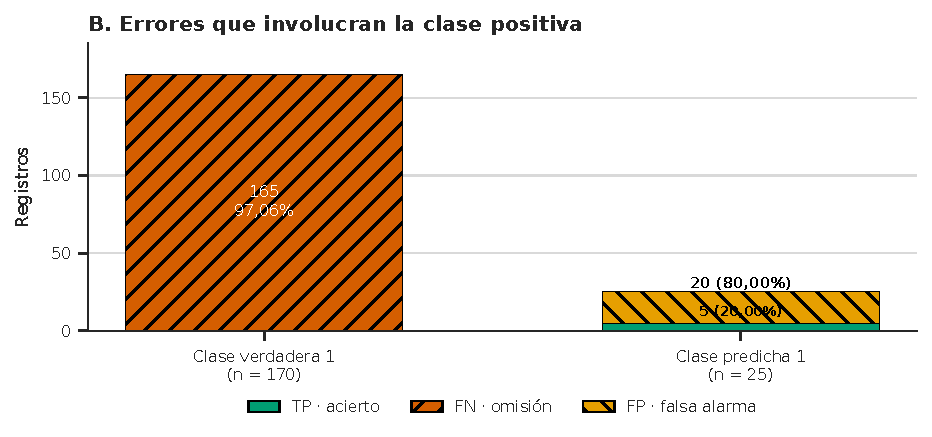
\includegraphics[width=0.82\textwidth]{output/figures/errores_clase_positiva.pdf}
\caption{Errores de clasificación de la clase peligrosa para el Decision Tree base, obtenidos mediante AI Studio.}
\label{fig:dt-errors}
\end{figure}

\begin{figure}[H]
\centering
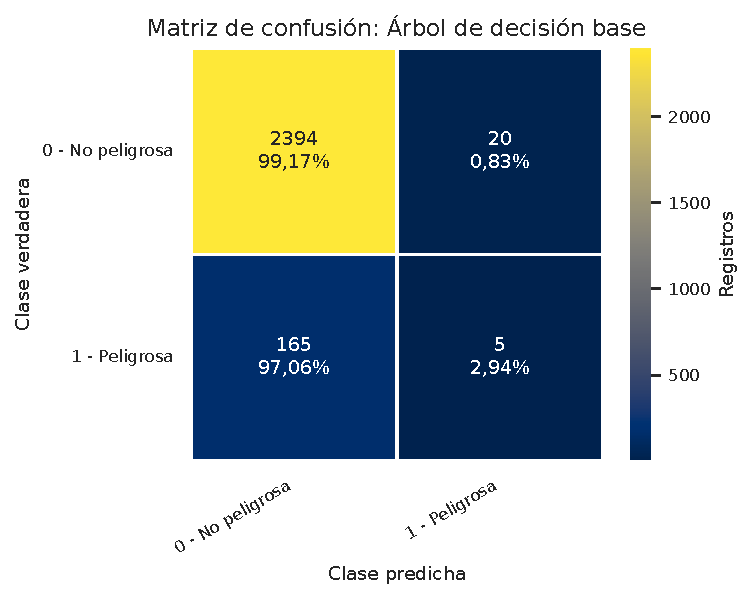
\includegraphics[width=0.70\textwidth]{output/figures/matriz_confusion_dt_base.pdf}
\caption{Matriz de confusión del Decision Tree base, con filas verdaderas y columnas predichas.}
\label{fig:dt-matrix}
\end{figure}

El resultado muestra que una exactitud cercana al 93\% puede coexistir con una cobertura muy baja de la clase peligrosa. En este caso, la métrica global resume principalmente el comportamiento sobre la clase 0, que constituye el 93,42\% de las instancias. Por eso, el análisis del árbol base debe centrarse menos en su exactitud aislada y más en el costo potencial de omitir casos de la clase 1.

\section{Segundo resultado empírico: Naive Bayes base}
Naive Bayes base obtuvo una exactitud de 84,75\% $\pm$ 4,31\% y un AUC (optimistic) de 0,761 $\pm$ 0,043, según AI Studio. Su exactitud es inferior a la del árbol de decisión base y también presenta una variabilidad mayor en la exactitud entre particiones. En cambio, la matriz muestra una detección considerablemente mayor de los casos de la clase 1.

La matriz total fue:
\begin{table}[H]
\centering
\caption{Matriz de confusión de Naive Bayes base.}
\label{tab:nb-base-matrix}
\begin{tabular}{lrr}
\toprule
& \textbf{Predicha 0} & \textbf{Predicha 1} \\
\midrule
\textbf{Verdadera 0} & 2120 & 294 \\
\textbf{Verdadera 1} & 100 & 70 \\
\bottomrule
\end{tabular}
\end{table}

Naive Bayes identifica correctamente 70 de los 170 registros peligrosos. Para lograrlo, clasifica como positivos 364 registros en total: 70 son verdaderos positivos y 294 son falsos positivos. El modelo también produce 100 falsos negativos, una cantidad inferior a la del árbol base, aunque no logra detectar todos los casos peligrosos.

Las métricas agregadas calculadas a partir de la matriz son precisión 19,23\%, recall 41,18\% y F1 26,22\%. El encabezado de AI Studio informa una precisión de 20,24\% $\pm$ 4,89\%, un recall de 41,20\% $\pm$ 6,84\% y un F1 de 26,80\% $\pm$ 5,24\%. Al igual que en el caso anterior, los valores agregados y los promedios del encabezado deben leerse como resúmenes complementarios del mismo procedimiento de validación.

\begin{figure}[H]
\centering
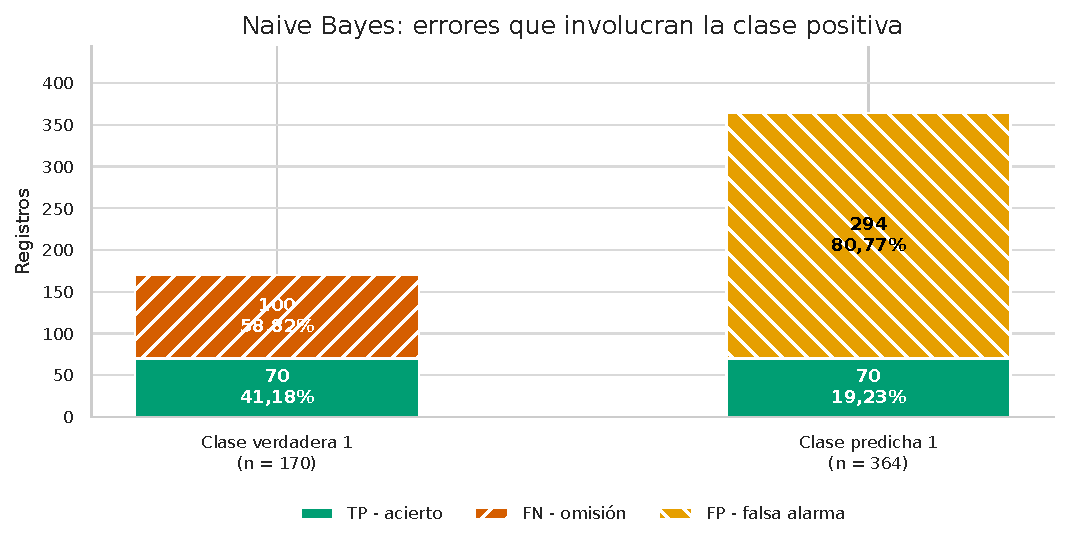
\includegraphics[width=0.82\textwidth]{output/figures/errores_clase_positiva_naive_bayes.pdf}
\caption{Errores de clasificación de la clase peligrosa para Naive Bayes base, obtenidos mediante AI Studio.}
\label{fig:nb-errors}
\end{figure}

\begin{figure}[H]
\centering
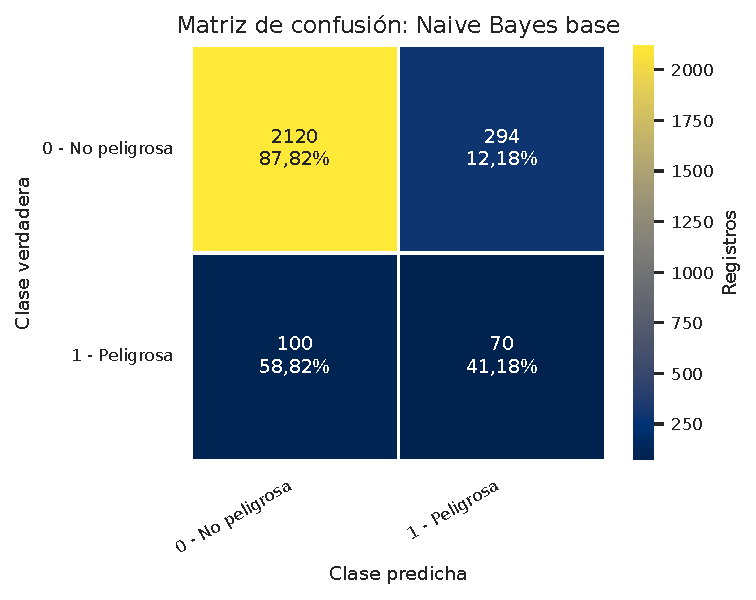
\includegraphics[width=0.70\textwidth]{output/figures/matriz_confusion_nb_base.pdf}
\caption{Matriz de confusión de Naive Bayes base, con filas verdaderas y columnas predichas.}
\label{fig:nb-matrix}
\end{figure}

El comportamiento de Naive Bayes evidencia el intercambio entre detección y falsas alarmas. Frente al árbol base, aumenta sustancialmente la cantidad de casos peligrosos detectados, pero también asigna la clase positiva a muchos registros que pertenecen a la clase 0. Por lo tanto, su menor exactitud no implica necesariamente un resultado menos útil si el objetivo prioritario es reducir la omisión de eventos peligrosos.

\section{Tercer resultado empírico: k-NN}
La evaluación de k-NN se realizó después de incorporar la normalización y de agrupar el preprocesamiento con el clasificador. La Tabla~\ref{tab:knn-k-selection} resume los resultados obtenidos para los cuatro valores candidatos de $k$. El criterio denominado ``AUC (optimistic)'' corresponde exactamente al indicador mostrado por AI Studio; no se lo presenta como AUC estándar ni se lo interpreta como equivalente a este último.

\begin{table}[H]
\centering
\caption{Selección del parámetro $k$ para k-NN.}
\label{tab:knn-k-selection}
\small
\begin{tabular}{@{}c c c c c c@{}}
\toprule
\textbf{$k$} & \textbf{Accuracy} & \shortstack{\textbf{AUC}\\\textbf{(optimistic)}} & \shortstack{\textbf{Precision}\\\textbf{clase 1}} & \shortstack{\textbf{Recall}\\\textbf{clase 1}} & \shortstack{\textbf{F1}\\\textbf{clase 1}} \\
\midrule
3 & 92,38\% & 0,892 & 26,32\% & 8,82\% & 13,22\% \\
5 & 93,07\% & 0,851 & 39,02\% & 9,41\% & 15,17\% \\
7 & 93,23\% & 0,825 & 40,00\% & 5,88\% & 10,26\% \\
9 & 93,23\% & 0,804 & 36,84\% & 4,12\% & 7,41\% \\
\bottomrule
\end{tabular}
\end{table}

Entre los valores evaluados, se seleccionó $k=5$ como configuración final de k-NN. Este valor maximiza simultáneamente el recall y el F1 de la clase 1: identifica 16 de los 170 registros peligrosos y obtiene un recall de 9,41\%. El valor $k=3$ alcanza el AUC (optimistic) más alto, 0,892, pero presenta una precisión de clase 1 de 26,32\% y un F1 de 13,22\%, inferiores a los de $k=5$. Por su parte, $k=7$ y $k=9$ conservan una exactitud similar o mayor, pero reducen la detección de la clase peligrosa. La selección de $k=5$ es, por lo tanto, una elección relativa entre los candidatos probados y no implica que el recall absoluto sea suficiente para un sistema operativo de alertas.

La matriz de confusión de la configuración seleccionada se presenta en la Tabla~\ref{tab:knn-k5-matrix}. La convención es la misma que en los modelos anteriores: las filas corresponden a la clase verdadera y las columnas a la clase predicha.

\begin{table}[H]
\centering
\caption{Matriz de confusión de k-NN con $k=5$.}
\label{tab:knn-k5-matrix}
\begin{tabular}{lrr}
\toprule
 & \textbf{Predicha 0} & \textbf{Predicha 1} \\
\midrule
\textbf{Verdadera 0} & 2389 & 25 \\
\textbf{Verdadera 1} & 154 & 16 \\
\bottomrule
\end{tabular}
\end{table}

La matriz muestra que el modelo seleccionado produce 25 falsos positivos y 154 falsos negativos. Por consiguiente, aunque k-NN mejora el recall y el F1 respecto de los otros valores de $k$ probados, todavía omite la mayoría de los registros de la clase peligrosa.

\section{Cuarto resultado empírico: regresión logística}
La regresión logística obtuvo una exactitud promedio de 87,89\% $\pm$ 1,31\% y un AUC (optimistic) de 0,758 $\pm$ 0,051. Para la clase 1, AI Studio informó una precisión promedio por partición de 25,69\% $\pm$ 3,64\%, un recall de 44,12\% $\pm$ 8,21\% y un F1 de 32,28\% $\pm$ 4,44\%.

La matriz de confusión acumulada fue:
\begin{table}[H]
\centering
\caption{Matriz de confusión de la regresión logística.}
\label{tab:logistic-matrix}
\begin{tabular}{lrr}
\toprule
 & \textbf{Predicha 0} & \textbf{Predicha 1} \\
\midrule
\textbf{Verdadera 0} & 2196 & 218 \\
\textbf{Verdadera 1} & 95 & 75 \\
\bottomrule
\end{tabular}
\end{table}

A partir de estos conteos, la precisión agregada de la clase 1 es 25,60\%, el recall agregado es 44,12\% y el F1 agregado es 32,40\%. Las pequeñas diferencias entre la precisión y el F1 agregados y sus respectivos promedios por partición se deben a que AI Studio promedia los resultados de los pliegues, mientras que las métricas agregadas se calculan una sola vez sobre los conteos acumulados. El modelo identificó 75 de los 170 registros peligrosos y dejó 95 falsos negativos.

\section{Comparación final de los cuatro modelos base}
La Tabla~\ref{tab:base-model-comparison} compara los cuatro algoritmos ejecutados. Para la precisión, el recall y el F1 de la clase 1 se utilizan valores agregados calculados a partir de las matrices de confusión totales. La exactitud y el AUC (optimistic) corresponden a los valores reportados por AI Studio; cuando la herramienta informó variabilidad entre particiones, se conserva el término $\pm$. Por tanto, no deben confundirse los promedios por pliegue con los cocientes derivados de los conteos acumulados.

\begin{table}[H]
\centering
\caption{Comparación final de los cuatro modelos base.}
\label{tab:base-model-comparison}
\small
\resizebox{\textwidth}{!}{%
\begin{tabular}{@{}lccccc@{}}
\toprule
\textbf{Modelo} & \textbf{Exactitud} & \shortstack{\textbf{AUC}\\\textbf{(optimistic)}} & \shortstack{\textbf{Precisión agregada}\\\textbf{clase 1}} & \shortstack{\textbf{Recall agregado}\\\textbf{clase 1}} & \shortstack{\textbf{F1 agregado}\\\textbf{clase 1}} \\
\midrule
Árbol de decisión & 92,84\% $\pm$ 0,27\% & 0,860 $\pm$ 0,041 & 20,00\% & 2,94\% & 5,13\% \\
Naive Bayes & 84,75\% $\pm$ 4,31\% & 0,761 $\pm$ 0,043 & 19,23\% & 41,18\% & 26,22\% \\
k-NN ($k=5$) & 93,07\% & 0,851 & 39,02\% & 9,41\% & 15,17\% \\
Regresión logística & 87,89\% $\pm$ 1,31\% & 0,758 $\pm$ 0,051 & 25,60\% & 44,12\% & 32,40\% \\
\bottomrule
\end{tabular}%
}
\end{table}

\begin{figure}[htbp]
\centering
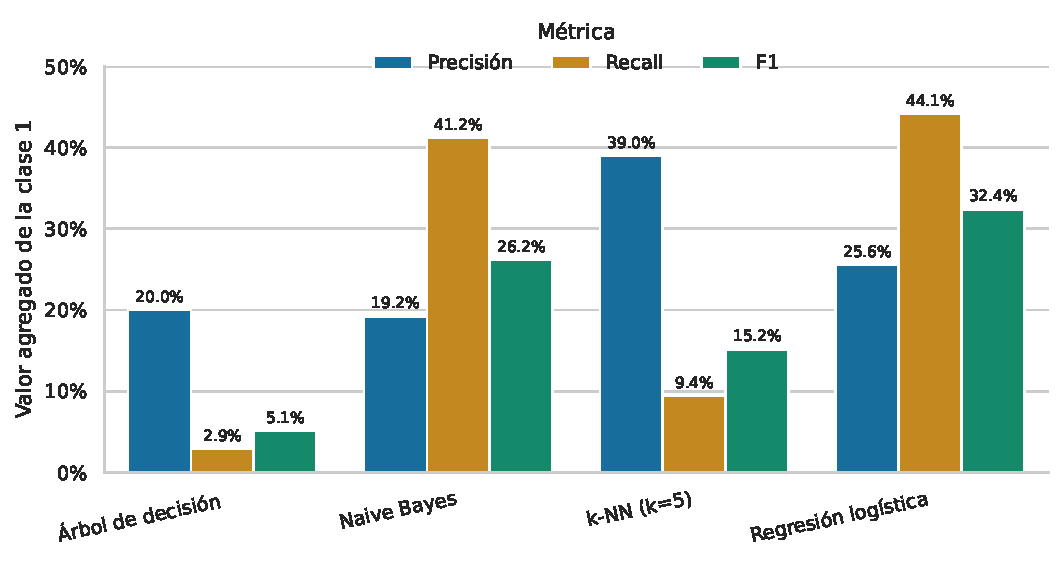
\includegraphics[width=0.96\textwidth]{output/figures/comparison_class1_metrics.pdf}
\caption{Comparación de la precisión, el recall y el F1 agregados de la clase 1 para los cuatro modelos base.}
\label{fig:comparison-class1-metrics}
\end{figure}

La Figura~\ref{fig:comparison-class1-metrics} hace visible que ningún modelo domina simultáneamente las tres métricas de la clase peligrosa. k-NN presenta la mayor precisión agregada, mientras que la regresión logística alcanza el mayor recall y F1. El árbol de decisión mantiene una cobertura muy baja de la clase 1 y Naive Bayes recupera una proporción considerable de positivos, aunque con menor precisión.

La matriz de cada modelo completa esta comparación: el árbol de decisión produjo 20 falsos positivos y 165 falsos negativos; Naive Bayes, 294 y 100; k-NN, 25 y 154; y la regresión logística, 218 y 95, respectivamente. Frente al árbol de decisión y a k-NN, la regresión logística aumenta la detección de eventos peligrosos a costa de un mayor número de falsos positivos. En cambio, frente a Naive Bayes mejora simultáneamente los verdaderos positivos (75 frente a 70), los falsos negativos (95 frente a 100), los falsos positivos (218 frente a 294) y la exactitud (87,89\% frente a 84,75\%).

\section[Interpretación conjunta de los resultados empíricos]{Interpretación conjunta de los resultados\\empíricos}
Los cuatro resultados empíricos permiten analizar el efecto del desbalance sobre la evaluación. El árbol de decisión base obtiene 92,84\% de exactitud, valor cercano a la proporción de la clase mayoritaria, pero su recall agregado de la clase 1 es 2,94\%. El resultado es consistente con un modelo que clasifica correctamente muchos registros no peligrosos y que, al mismo tiempo, deja sin detectar la mayor parte de los casos peligrosos.

Naive Bayes base presenta un comportamiento diferente. Su exactitud de 84,75\% es menor, pero su recall agregado alcanza 41,18\% y su F1 agregado 26,22\%, frente a 5,13\% del árbol. La mejora en detección se obtiene a costa de 294 falsos positivos. En un escenario donde una alarma adicional es aceptable frente a la omisión de un evento, este intercambio podría ser preferible; en un escenario donde las falsas alarmas generan interrupciones costosas, la decisión podría ser distinta.

El k-NN seleccionado con $k=5$ alcanza una exactitud de 93,07\%, un AUC (optimistic) de 0,851, una precisión de clase 1 de 39,02\%, un recall de 9,41\% y un F1 de 15,17\%. En comparación con el árbol base, identifica más casos peligrosos, aunque todavía deja 154 falsos negativos. Estos resultados muestran que la normalización y la selección de $k$ permiten configurar el modelo de manera reproducible, pero no eliminan por sí solas la dificultad asociada al desbalance.

La regresión logística alcanza el mayor recall y el mayor F1 agregados de los cuatro modelos base: 44,12\% y 32,40\%, respectivamente. Esta mejora implica detectar 75 casos peligrosos, frente a 70 de Naive Bayes, 16 de k-NN y 5 del árbol. Frente al árbol de decisión y a k-NN, la mayor cobertura se obtiene a costa de más falsos positivos y de una exactitud inferior. Frente a Naive Bayes, en cambio, la regresión logística mejora simultáneamente los verdaderos positivos (75 frente a 70), los falsos negativos (95 frente a 100), los falsos positivos (218 frente a 294) y la exactitud (87,89\% frente a 84,75\%). Por lo tanto, el costo en falsas alarmas no aumenta respecto de todos los modelos, sino únicamente respecto de las alternativas más conservadoras en la predicción de la clase peligrosa.

El AUC (optimistic) también debe leerse con cautela. Los procesos RMP disponibles activan este criterio en \textit{Performance} y desactivan el AUC estándar; por ello, la denominación se conserva de forma consistente. El archivo disponible que contiene Naive Bayes también incluye un operador SMOTE activo, por lo que permite verificar la configuración del criterio, pero no reproducir de manera aislada la ejecución base informada. Asimismo, el indicador no fija por sí mismo un umbral operativo ni representa directamente la cantidad de falsos negativos que se aceptaría en producción. Estos valores no fueron recalculados a partir de predicciones exportadas, de modo que su comparación se limita al criterio homónimo reportado por AI Studio.

Por estas razones, la regresión logística constituye el modelo base más favorable si se priorizan el recall y el F1 de la clase peligrosa, pero no puede declararse automáticamente como solución operativa. La selección definitiva requiere explicitar el costo relativo de falsos negativos y falsos positivos, revisar el umbral de decisión y evaluar la estabilidad temporal. Como extensión complementaria, podrá estudiarse SMOTE por separado y únicamente dentro de los pliegues de entrenamiento; no se lo presenta como parte de los cuatro resultados base ya ejecutados.

\section{Fuente inicial}
Sikora, M., y Wrobel, L. (2010). \textit{Seismic-Bumps}. UCI Machine Learning Repository.\\
\url{https://archive.ics.uci.edu/dataset/266/seismic+bumps}\\
Chawla, N. V., Bowyer, K. W., Hall, L. O., \& Kegelmeyer, W. P. (2002). \textit{SMOTE: Synthetic Minority Over-sampling Technique}. Journal of Artificial Intelligence Research, 16, 321--357. URL: \url{https://doi.org/10.1613/jair.953}
\end{document}
